% Created 2025-07-10
% Intended LaTeX compiler: pdflatex
\documentclass[11pt,a4paper]{article}

% ────────────── Paquetes básicos ──────────────
\usepackage[utf8]{inputenc}
\usepackage[T1]{fontenc}
\usepackage[spanish]{babel}
\usepackage{graphicx,grffile}
\usepackage{longtable,wrapfig,rotating}
\usepackage[normalem]{ulem}
\usepackage{amsmath,amssymb,textcomp}
\usepackage{tabularx,lastpage,enumitem}
\usepackage[table,xcdraw]{xcolor}
\usepackage[left=2cm,right=2.5cm,top=2.5cm,bottom=2.5cm]{geometry}
\usepackage{hyperref}
\usepackage{siunitx}

% ────────────── Comandos de metadatos ─────────
\newcommand*{\autor}[1]{\def\authorname{#1}}
\newcommand*{\titulo}[1]{\def\@title{#1}\def\ttitle{#1}}
\newcommand{\versionActual}{A}
\newcommand{\fechaA}{10/07/2025}
\newcommand{\docCode}{\normalsize RETRO\_GAME-RH versión \versionActual}
\newcommand{\fechaActual}{\fechaA}

\titulo{Videojuego portátil inspirado en consolas retro}
\autor{Lic. Jezabel Danon}

% ────────────── Encabezado / pie ──────────────
\usepackage{fancyhdr}
\fancyhf{}
\pagestyle{fancy}
\lhead{
\includegraphics[width=3.5cm]{../Figuras/logoFIUBA.pdf}}
\rhead{\normalsize\textbf{\@title}\\Especificación de requisitos de hardware\\\docCode}
\setlength{\headheight}{42pt}
\setlength{\footskip}{25pt}
\cfoot{\normalsize Página \thepage{} de \pageref{LastPage}}
\renewcommand{\headrulewidth}{1pt}
\renewcommand{\footrulewidth}{0.4pt}

% ────────────── Hipervínculos ─────────────────
\hypersetup{
  colorlinks=true,
  linkcolor=black,
  urlcolor=blue,
  pdftitle={\@title},
  pdfauthor={\authorname},
  pdflang={es}
}

% ────────────── Documento ─────────────────────
\begin{document}

% ----- Portada -----
\begin{titlepage}
  \centering
  
\includegraphics[width=.7\textwidth]{../Figuras/logoFIUBA.pdf}\par
  \vspace{1cm}
  {\Huge\textbf{\ttitle}}\par
  \vspace{1.5cm}
  {\Large\itshape Especificación de requisitos de hardware (ERH)\par}
  \vspace{3cm}
  \flushleft
  {\normalsize Autor:}\par
  {\Large \authorname\ (jezabel.danon@gmail.com)}\par
  \vspace{1.5cm}
  {\scshape\LARGE \fechaActual}\par
  {\scshape\LARGE Versión \versionActual}\par
  \vfill
  \centering
  \textit{}%Basado en la guía IEEE 1233-1998 y alineado con la ERS RETRO\_GAME-RS.}
\end{titlepage}

\clearpage
\tableofcontents
\clearpage

% ---------- 1 Introducción ----------
\section{Introducción}

\subsection{Propósito}
\begin{enumerate}
  \item El propósito de este documento es detallar los requisitos de hardware necesarios
para el desarrollo del dispositivo \textit{\ttitle}.  
  \item Sirve como referencia para los equipos de ingeniería electrónica,
integración, verificación y compras.
\end{enumerate}

\subsection{Alcance}
\begin{enumerate}
  \item El documento cubre todos los bloques electrónicos del prototipo: fuente de alimentación, unidad de procesamiento (MCU STM32), módulos de entrada/salida, audio, vibración y pantalla.
  \item Quedan fuera de alcance los aspectos de diseño y montaje de PCB, así como el diseño mecánico de la carcasa u otros componentes externos.
\end{enumerate}


\subsection{Definiciones, acrónimos y abreviaturas}
\begin{description}[labelwidth=2cm,labelindent=0.6cm]
  \item[MCU] Microcontroller Unit
  \item[RTOS] Real-Time Operating System
  \item[EEPROM] Electrically Erasable Programmable Read-Only Memory
  \item[TFT] Thin-Film Transistor display
  \item[BOM] Bill of Materials
\end{description}

\subsection{Referencias}
\begin{enumerate}
  \item IEEE 1233-1998 - Guide for Developing System Requirements Specifications.
  \item Especificación de requisitos de software: RETRO\_GAME-RS-vA.
  \item href{https://drive.google.com/file/d/1C3vEYR8wME6EzlZVVC-gT2u86dwnoZA-/view?usp=sharing}{Plan de proyecto del trabajo práctico final} para la \textit{Carrera de Especialización en Sistemas Embebidos} (RETRO\_GAME-PP-v5). 
  \item Especificaciones de requisitos de hardware: RETRO\_GAME-RH-vA.
\end{enumerate}

% ---------- 2 Visión general del sistema ----------
\section{Visión general del sistema}

\subsection{Descripción general}
El hardware se organiza en cinco grupos:

\begin{enumerate}
  \item \textbf{Unidad de procesamiento} - placa STM32 NUCLEO-F446RE.
  \item \textbf{Alimentación} - módulo conversor 9 {\si\volt} → 5{\si\volt} /{3.3}{\si\volt} + batería.
  \item \textbf{Interfaces de entrada}
  \begin{itemize}
    \item joystick analógico KY-023, 
    \item botones tact switch, 
    \item acelerómetro del MPU-6500.
  \end{itemize}
  \item \textbf{Interfaces de salida} 
  \begin{itemize}
    \item pantalla TFT ST7735R, 
    \item parlante 8 Ω 1 W (con amplificador LM386), 
    \item motor de vibración con controlador DRV2605L.
  \end{itemize}
  \item \textbf{Memoria externa} - EEPROM SPI 25LC256.
\end{enumerate}

% (Opcional: incluye aquí tu diagrama de bloques si lo deseas)
\begin{figure}[h]
  \centering
  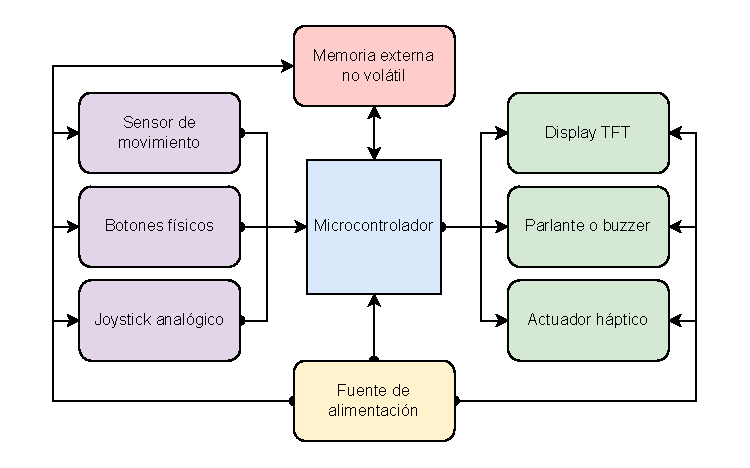
\includegraphics[width=.9\linewidth]{../Figuras/diagrama_bloques_proyecto.pdf}
  \caption{Diagrama de bloques de alto nivel.}
\end{figure}

% ---------- 3 Requisitos funcionales de hardware ----------
\section{Requisitos funcionales de hardware}

\begin{description}[labelindent=0.5cm]
  \item[\texttt{RETRO\_GAME-RH-REQ0001:}] El hardware será montado sobre protoboard sin necesidad de soldadura permanente. Todos los módulos seleccionados deben poseer encapsulado tipo DIP o header estándar compatible.
  
  \item[\texttt{RETRO\_GAME-RH-REQ0002:}] El sistema deberá alimentarse mediante una fuente de corriente continua.

  \item[\texttt{RETRO\_GAME-RH-REQ0003:}]  El sistema deberá incorporar un sensor de inclinación de al menos dos ejes.

  \item[\texttt{RETRO\_GAME-RH-REQ0004:}] Se deberá contar con un joystick analógico de dos ejes. 

  \item[\texttt{RETRO\_GAME-RH-REQ0005:}] Se deberán proveer al menos cuatro botones tipo tact-switch, conectados a entradas digitales del microcontrolador. 

  \item[\texttt{RETRO\_GAME-RH-REQ0006:}] El sistema deberá incluir una pantalla que permita representar texto e imágenes. 

  \item[\texttt{RETRO\_GAME-RH-REQ0007:}] El sistema deberá ser capaz de generar salidas sonoras para retroalimentación. 

  \item[\texttt{RETRO\_GAME-RH-REQ0008:}] El sistema deberá incluir un motor de vibración para retroalimentación háptica. 

  \item[\texttt{RETRO\_GAME-RH-REQ0009:}] El sistema deberá permitir guardar y restaurar partidas mediante una memoria no volátil. 
\end{description}

% ---------- 4 Requisitos no func ----------
\section{Requisitos no funcionales de hardware}

\subsection{Alimentación}
\begin{description}[labelindent=0.5cm]
  \item[\texttt{RETRO\_GAME-RH-REQ0010:}] Se requiere una tensión estabilizada de {3.3}{\si\volt} ±5 \% y {5}{\si\volt} ±5 \%.
  \item[\texttt{RETRO\_GAME-RH-REQ0011:}] Corriente pico disponible: 800{\si\mA}.
\end{description}
% Si querés un dato real:
% Calculá el peor caso de cada bloque (según hojas de datos):
% Pantalla TFT ST7735R retroiluminada ≈ 60 mA
% LM386 a 1 W con 8 Ω ≈ 350 mA pico (eficiencia típica)
% Motor ERM 3 V (arranque) ≈ 120 mA
% STM32 a 180 MHz + periféricos ≈ 50-70 mA
% Otros (MPU-6500, EEPROM, LEDs) < 20 mA
% Suma los picos simultáneos que puedan ocurrir (por ejemplo, audio + pantalla + MCU). En mi borrador redondeé a ~600 mA y añadí un 30 % de margen de diseño ⇒ ≈ 800 mA.
% Conclusión: 800 mA es solo un número de referencia. Sustituilo por el valor real que te dé tu cálculo de potencia con margen de ingeniería (usualmente 20-30 %).

\subsection{Procesamiento}
\begin{description}[labelindent=0.5cm]
  \item[\texttt{RETRO\_GAME-RH-REQ0012:}] MCU Cortex-M4 a 180 MHz, 512 kB Flash, 128 kB SRAM.
\end{description}

\subsection{Entradas}
\begin{description}[labelindent=0.5cm]
  \item[\texttt{RETRO\_GAME-RH-REQ0013:}] Joystick analógico KY-023 → MCU ADC (2 canales, 12 bit).
  \item[\texttt{RETRO\_GAME-RH-REQ0014:}] Cuatro botones tipo tact switch conectados a GPIO con resistencias pull-up externas; debounce por software.
  \item[\texttt{RETRO\_GAME-RH-REQ0015:}] Sensor MPU-6500 (I\textsuperscript{2}C @ {400}{\si\kHz}, genera interrupción “data ready” a {100}{\si\hertz}.
\end{description}

\subsection{Salidas}
\begin{description}[labelindent=0.5cm]
  \item[\texttt{RETRO\_GAME-RH-REQ0016:}] Pantalla TFT 1.8 inch ST7735R; interfaz SPI a {24}{\si\MHz}; DMA para transferir {128 x 160 x 16} bits por cuadro.
  \item[\texttt{RETRO\_GAME-RH-REQ0017:}] Audio: parlante 8 {\si\ohm} 1 {\si\watt} amplificado por LM386; señal PWM entre \qtyrange{20}{50}{\kHz}.
  \item[\texttt{RETRO\_GAME-RH-REQ0018:}] Vibración: motor ERM {3}{\si\volt}; excitado por DRV2605L (I\textsuperscript{2}C, patrones integrados).
\end{description}

\subsection{Persistencia}
\begin{description}[labelindent=0.5cm]
  \item[\texttt{RETRO\_GAME-RH-REQ0019:}] Memoria SPI 25LC256 (256kb).
\end{description}

% ---------- 5 Requisitos mecánicos ----------
% \section{Requisitos mecánicos}

% \begin{itemize}
%   \item PCB simple de \si{82 x 56}{\milli\metre}, FR-4,
%         espesor \si{1.6}{\milli\metre}.
%   \item Altura máxima componente: \si{8}{\milli\metre}
%         (para caber en carcasa impresa en 3D).
% \end{itemize}

% ---------- 6 Lista preliminar de materiales (BOM) ----------
\section{Lista preliminar de materiales (BOM)}

\begin{longtable}{|c|p{4cm}|p{4.5cm}|c|p{3cm}|}
\hline
\rowcolor[HTML]{C0C0C0}
\textbf{Ítem} & \textbf{Componente} & \textbf{Descripción} & \textbf{Cant.} & \textbf{Notas} \\
\hline
1  & STM32 NUCLEO-F446RE             & Placa de desarrollo MCU Cortex-M4 @180 MHz         & 1 & Unidad de procesamiento \\ \hline
2  & ST7735R TFT 1.8"     & Pantalla TFT 128x160 px SPI                         & 1 & Con back-light LED \\ \hline
3  & 25LC256                         & EEPROM SPI 256kb                     & 1 & SOIC-8 \\ \hline
4  & DRV2605L                        & Controlador háptico I\textsuperscript{2}C           & 1 &  \\ \hline
5  & Motor ERM {3}{\si\volt}         & Vibrador cilíndrico {44,000} rpm               & 1 & Montaje con cinta \\ \hline
6  & Speaker 8 Ω 1 W                 & Parlante dinámico Ø {28}{\si\mm}          & 1 &  \\ \hline %En caja acústica
7  & LM386                            & Amplificador audio {0.7}{\si\watt}                 & 1 & SO-8 \\ \hline
8  & GY-521 (MPU-6500)               & Módulo acelerómetro/giroscopio                     & 1 & I\textsuperscript{2}C, 3.3 V \\ \hline
9  & Módulo DC-DC 9 V → 5/3.3 V      & Regulador step-down dual-rail                      & 1 & Salida {1.2}{\si\ampere} máx. \\ \hline
10 & Joystick analógico KY-023       & Potenciómetro bi-eje + botón                       & 1 & \\ \hline
11 & Tact switch (botón)             & Pulsador THT {4}{\si\mm}                  & 4 &  \\ \hline
12 & Protoboard (400 pts)            & Panel prototipado                          & 1 &  \\ \hline
13 & Cables jumper M-F / M-M         & Conductores dupont {20}{\si\cm}           & 30 & Conexión del prototipo \\ \hline
\end{longtable}

% ---------- 7 Verificación y validación ----------
\section{Verificación y validación}

\subsection{Objetivo}
Confirmar que cada requisito de hardware (RH-1.1 a RH-1.9) se
cumple en el prototipo y que, en conjunto, el sistema satisface la
función de juego portátil sin fallos perceptibles para el usuario
final.

\subsection{Enfoque general}
\begin{enumerate}[label=\alph*)]
  \item \textbf{Verificación} = “¿lo construí bien?”  
        Se aplican inspección visual, lectura de hoja de datos y pruebas
        funcionales de laboratorio.
  \item \textbf{Validación} = “¿con esto cumplo la necesidad?”  
        Se realizan ensayos de uso real (sesión de juego, demo),
        demostraciones en vídeo y pruebas de estrés.
  \item Cada ensayo se documentará con: fecha, responsable, equipo de
        medida, pasos, resultados y evidencia (fotos / capturas UART).
\end{enumerate}

\subsection{Matriz de V\&V}
\begin{longtable}{|p{2cm}|p{5.3cm}|p{4.7cm}|p{4.7cm}|}
\hline
\rowcolor[HTML]{C0C0C0}
\textbf{Req.\ ID} &
\textbf{Método de verificación} &
\textbf{Criterio de aceptación} &
\textbf{Método de validación} \\ \hline
REQ0001 (Montaje) &
Comparar el cableado real con el esquema; revisar soldaduras
o posición en protoboard. &
No hay conexiones faltantes ni invertidas. &
Inspección cruzada del esquema y fotografías macro del
prototipo. \\ \hline
REQ0002 (Alimentación a batería) &
Prueba de encendido con todos los
periféricos y registro de tensión durante
el arranque. &
El sistema arranca sin reinicios; V\textsubscript{out}
3.3 V ±5 \%. &
Sesión de juego continua de
45 min con batería de 9 V;
sin cortes ni reinicios. \\ \hline
REQ0003 (Acelerómetro) &
Leer ejes X/Y por UART con código de prueba;
comprobar hoja de datos (al menos 2 ejes). &
Lecturas varían suavemente al inclinar
el dispositivo ±90°. &
Mover el prototipo en varios
ángulos y observar que los
valores reportados son coherentes y estables. \\ \hline
REQ0004 (Joystick analógico) &
Enviar por UART los valores de ambos
potenciómetros al desplazar la palanca. &
Cada eje entrega un rango continuo
0-4095\,(ADC 12 bit). &
El usuario mueve la palanca y
verifica, en pantalla o terminal,
respuesta proporcional sin zonas muertas. \\ \hline
REQ0005 (Botones) &
Programa de test que detecte flancos
y muestre su estado. &
Todos los botones generan evento
“presión” y “liberación” < 20 ms. &
Prueba interactiva: pulsar
cada botón; la acción asignada
se ejecuta sin retardos ni rebotes
perceptibles. \\ \hline
REQ0006 (Pantalla TFT) &
Secuencia de inicialización + demo
de texto, líneas y sprites. &
La pantalla responde a comandos,
sin parpadeos ni líneas muertas. &
Inspección visual: gráficos se ven
correctamente durante una escena del
demo de juego. \\ \hline
REQ0007 (Audio) &
Señal PWM de prueba → LM386 →
parlante &
Nivel audible sin distorsión
excesiva. &
Reproducir efecto “jingle”;
usuarios confirman claridad y volumen adecuados. \\ \hline
REQ0008 (Vibración ERM) &
Activar 2 patrones del DRV2605L
y comprobar corriente. &
El motor arranca en < 100 ms y
genera patrón de vibración. &
Usuario percibe la vibración. \\ \hline
REQ0009 (EEPROM) &
Escribir y leer un bloque de prueba;
ciclar 10 veces. &
Los datos leídos coinciden byte-a-byte
con lo escrito; sin errores CRC. &
Guardar datos de partida dummy, cortar
alimentación al menos 1 h, volver a
cargar - la partida se recupera idéntica. \\ \hline
\end{longtable}

\subsection{Trazabilidad}
Cada requisito REQ000x se vincula al resultado de su prueba:
\begin{itemize}
  \item \texttt{TEST\_BAT01} → REQ0002  
  \item \texttt{TEST\_JOY01} → REQ0004  
  \item \texttt{TEST\_EEP01} → REQ0009  
\end{itemize}
Los reportes se almacenan en
\texttt{docs/TEST\_REPORTS/\<fecha\>} con evidencia fotográfica y
logs UART.

\subsection{Criterio de aceptación global}
El hardware se considera “listo para integración con firmware” cuando:
\begin{enumerate}
  \item El 100 \% de los casos de prueba arriba listados pasan sin
        incidencias.
  \item La validación de juego completo (sesión > 45 min, batería)
        transcurre sin reinicios ni fallos de periféricos.
\end{enumerate}

% ---------- 8 Aprobaciones ----------
% \section*{Firmas de aprobación}
% \vspace{2cm}
% \begin{tabularx}{\textwidth}{X X}
% \hrulefill & \hrulefill \\
% Autor & Revisor técnico \\
% \end{tabularx}

\end{document}
